%% Support sites:
%% http://www.michaelshell.org/tex/ieeetran/
%% http://www.ctan.org/pkg/ieeetran
%% and %% http://www.ieee.org/

\documentclass[conference]{IEEEtran}
\usepackage{lipsum}
\usepackage{graphicx}
\usepackage{amsmath}
\usepackage{array}
\usepackage{url}
\usepackage[noadjust]{cite}

%\usepackage{natbib}
\usepackage{dtklogos} % for BibTeX stylized logo

\usepackage{amssymb}

% correct bad hyphenation here
\hyphenation{op-tical net-works semi-conduc-tor}

% adjust spaces in asmath userpackage
\interdisplaylinepenalty=2500

\begin{document}
\title{Convex Optimization for \\Holistic Mechatronic System Design}

%%%%%%%%%%%%%% begin authors %%%%%%%%%%%%%% 
\author{\IEEEauthorblockN{Yuchao Li}
\IEEEauthorblockA{School of Mechanic and \\Mechatronic Engineering\\
Royal Institute of Technology\\
Stockholm, Sweden\\
Email: Yuchao@kth.se}
\and
\IEEEauthorblockN{Anqing Duan}
\IEEEauthorblockA{School of Mechanic and \\Mechatronic Engineering\\
Royal Institute of Technology\\
Stockholm, Sweden\\
Email: Anqingd@kth.se}
\and
\IEEEauthorblockN{Alexander Gratner}
\IEEEauthorblockA{School of Mechanic and \\Mechatronic Engineering\\
Royal Institute of Technology\\
Stockholm, Sweden\\
Email: Gratner@kth.se}}
%%%%%%%%%%%%%% end authors %%%%%%%%%%%%%%%%

\maketitle %\IEEEpeerreviewmaketitle

%%%%%%%%%%%%%% abstract %%%%%%%%%%%%%
\begin{abstract}
\lipsum[1]
\end{abstract}
%%%%%%%%%%%%%% end abstract %%%%%%%%%%%%%%%

%%%%%%%%%%%%%% begin introduction %%%%%%%%%
\section{Introduction}

The current trend in research related to early design optimization of mechatronic systems is to use genetic algorithms to minimize the objective functions, but these approaches suffers from the potential disadvantages of genetic algorithms which could be avoided by using the convex optimization approach discussed in this paper. The multidisciplinary nature of mechatronic systems, which could be characterised as systems with synergistic integrations of mechanical engineering with electronics and intelligent computer control \cite{MechatronicsWWHHarashima}, makes early design optimization a difficult process. Optimizations are often done in the latter detailed design phases \cite{EngineeringDesign} whereas early design decisions becomes a limiting factor. Research on the topic of optimization in early design stages for mechatronic systems has presented both holistic and non-holistic approaches which share the common feature of using genetic algorithms, either as a complement or as a standalone solver. The disadvantages of GA when it comes to accuracy and computation time justifies research on applying disciplinary convex optimization.


\par
Optimizing mechatronic systems using genetic algorithms has been widely explored by researchers today. Hammadi et al. \cite{Hammadi2012, Hammadi2014} propose an emergent multi-agent approach where the system is decomposed into smal sub-systems (or agents) that in turn is optimized using the genetic algorithms NSGA II. Another approach that uses NSGA II is proposed by Guizani \cite{Guizani2014} where a partitioning method is utilized to decompose the mechatronic system and classification of the interactions between partions are done. An approach developed by Seo \cite{Seo2003} and further developed by Behbahani \cite{Behbahani2013, Behbahani2014} uses a two loop optimization process which incorporates genetic algorithms and bond graphs in an outer loop to optimize system topology and genetic programming in an inner loop to fin the elite solution within the optimal topology. The research in this paper will be based upon the work done by Malmquiest et al. \cite{malmquist2015tool}, they introduce a tool called IDIOM for holistic optimization of mechatronic design concept by utilizing genetic algorithms.

\par
The IDIOM framework developed by Malmquist et al. extends on the Roos \cite{roos2007} on a research on a methodology for integrated design and mechatronic servo systems. In his research, Roos reflects on the choice of using genetic algorithms to optimize the servo systems by stating that "The drawback of this method for system optimization is that it is computationally intensive and that there exists no mathematical proof that it actually finds the true optimum". This statement justifies the exploration of other optimization techniques which could provide true optimizations in a less computationally intensive manner, and for which convex optimization has been chosen. Disciplinary convex programming is a methodology developed by Grant et al. \cite{gb08} which purpose, according to the authors, is to "allow much of the manipulation and transformation required to analyse and solve convex programs to be automated". The methodology originates from procedures taken by those who regularly study convex optimization problems and has been implemented in the modelling framework called \textit{CVX} \cite{cvx} which serves as a package for specifying and solving convex programs.

\par
The argument made by Roos serve as a starting point in the research presented in this report. It challenges the current trend of using evolutionary algorithms when optimizing the design of mechatronic systems and could provide a optimization approach that is less computationally expensive and more accurate. 

\par
The remainder of this paper will introduce the previous work done by Malmquist et al. of which this study aim to extend on. Paragraph 3 describes the method used when applying convex optimization to the mechatronic system. Finally, paragraph 4 introduces a case study where a system optimization is performed, and compared to the results obtained by Malmquist et al., of a mechatronic system composed of a motor, planetary gear and a load.  



VIMTESTLOLOLOLOL \cite{Mechatronics}
%%%%%%%%%%%%%% end introduction %%%%%%%%%%%

%%%%%%%%%%%%%% begin Previous work %%%%%%%%%
\section{Previous Work}
Roos presented a methodology for the optimal design methodology\cite{roos2007}. According to his proposed methodology, an optimal mechatronic servo system consisting of a motor, planetary gear transmission and load can be achieved regarding system volume, weight and efficiency. The physical system configuration is shown in fig ???. Roos built various dimensioning models for the physical system upon the most critical constraints and designed the corresponding controller by time expensive simulation for minimized control error so that the complete system would be designed at the very early design phase. However, Roos$'$ methodology treats the static model and the dynamic model separately relying on two optimization loops, so the methodology is not very holistic. In fact, only one fixed system configuration: servo actuator was considered and could only be optimized mainly for a single objective in his methodology.

Malmquist et al. extended Roos$'$ work further. A prototype software tool was developed for implementing the methodology. The software allows for arbitrary system configuration including PMDC motor, planetary gear, harmonic drive, solid shaft, linear timing belt drive, load as well as full state feedback controller and multiple objectives can be optimized. With these elementary components, Malmquist presented design examples of haptic steering wheel and two axis gantry system. The methodology is completed to some extent and shows applicable potential to solve more general engineering problems compared with Roos.

The modeling part in Malmquist$'$s work also includes static model and dynamic model. The static model is built for each component based on the critical constraints of the component using objective-relevant design variables and can reflect the relationship between the capability of the component and its design variables. The model is scalable according to the required load. The complexity of the model is aimed at as low as possible so they did not use FEM-analysis for the reason of time efficiency.

The dynamic model in Malmquist$'$s work is used to evaluate the dynamic performance such as maximum integrated square error, maximum error and overshoot etc. Usually dynamics evaluation involves simulation and that would increase complexity as well as time consumption. The method proposed by Malmquist is that the dominant frequencies of the input signal are identified by applying Fourier transforms and
a series of sinusoidal waves would be used to mimic the input signal. Their corresponding outputs would be calculated based on the transfer function separately considering the frequency dependent gain and phase shift. The sum of all the individual output is regarded as the approximation of the time domain response. The transfer function is determined symbolically outside the optimization loop for the reason of time efficiency. During the optimization process of the dynamic part, the controller design without satisfying the dynamic requirements would be rejected. In addition, when the physical system is implemented with a controller, the static model derived earlier might be needed to be checked if it also fulfills the requirements of the dynamic behavior. Thus, a dimensioning factor is introduced to over- or under-dimension the static model so that an optimum could be obtained with both the static and dynamic properties taken into consideration.      

The optimization method employed by Malmquist is genetic algorithm, which is one of the most widely used evolutionary methods. It is a non-gradient based optimization. The algorithm is inspired by the Darwinian principle of natural selection. The possible solution with design variables can be compared to an individual with a number of genes. The optimum would be reached after breeding several generations. This method can handle a diverse range of problems but at a cost of low computation efficiency. So replacing it with a more efficient optimization method such as convex optimization is worth being studied further.
%%%%%%%%%%%%%% end Previous work %%%%%%%%%%%

%%%%%%%%%%%%%% begin Optimization approach %%%%%%%%%
\section{Optimization Approach}
In this section, we present general approach to convert a optimization problem of mechtronic product design to be the format of geometric programming. Some basics regarding convex optimization and geometric programming are introduced first. They are followed by three methods for construction of posynomial constraints for static properties of the system. Constraints regarding dynamic performance are interpreted in the end. 

\subsection{Mathematical Preliminaries}
The following introduction regarding convex optimization mainly come from \cite{boyd2004convex}. Note that the notations for different functions and sets will be used in later discussions. Before bringing the definition of convex optimization, we need to introduce what convex set and convex function are. A set $C$ is a convex set if for any two elements $x_1, x_2 \in C$, $\theta x_1+(1-\theta) x_2\in C$ holds for any $\theta \in \left[0,1\right]$. If the set $C$ represents a geometric region, any line segments defined by points which belong to $C$ shall be in the set. A function $f : \mathbf{R^n} \to \mathbf{R}$ is convex if \textbf{dom} $f$ is a convex set and any chord between any two points on $f$ lies above the graph of $f$. Based on the definition of convex function, a convex optimization (CO) problem is defined as 
\begin{align}
\begin{split}
\label{eq:problem}
\text{minimize} \quad  & f_0(x) \\
\text{subject to} \quad & f_i(x) \leq 0,\quad i=1,\ldots,m\\
                  & h_i(x) = 0,\quad i=1,\ldots,p
\end{split}
\end{align}
where all the functions in \ref{eq:problem} are convex functions. $f_0(x)$ is named as objective function, $f_i(x)$ inequality constraint and $h_i(x)$ equality constraint. Although it is now a mature technique to solve a CO problem, it is not easy to formulate objective and constraint functions as convex ones. In the case of mechatronic system design, some typical objective functions, such as volume of the system, are not convex functions and not allowed to be manipulated. However they do follow polynomial form. Luckily, it is still possible to take the advantage of CO technique if those optimization problems can be formulated as another classic form, which is geometric programming (GP).

Before discussion about GP, we need to introduce the form GP follows. A monomial function is defined as \ref{eq:monomial}
\begin{equation}
\label{eq:monomial}
f(x)=cx_1^{a_1}x_2^{a_2}\cdots x_n^{a_n}, \quad \mathbf{dom} \, f=\mathbf{R_{++}^n}
\end{equation}
where $c$ is positive and $a_i$ can be any real number. A posynomial function is a sum of monomials, which is 
\begin{equation}
\label{eq:posynomial}
f(x)=\sum_{k=1}^K c_kx_1^{a_{1k}}x_2^{a_{2k}}\cdots x_n^{a_{nk}}, \quad \mathbf{dom} \, f=\mathbf{R_{++}^n}
\end{equation}
A GP problem follows the same format as \ref{eq:problem}, except that objective and inequality constraints are posynomials and equality constraints are monomials. In fact, by conducting variable substitution, it is easy to show a GP problem can be transferred as a CO problem \cite{boyd2004convex}. 

In order to formulate an optimization as GP, we don't need to verify if a function is convex or not. Instead, we only need to make sure both objective and constraint functions follow either monomial or posynomial forms. In this way, it is avoided to manipulate functions to be convex and it provides a well defined principle for researchers to create constraints.

\subsection{Proposed Modeling Approach for Static Constraints}
GP is considered to be promising in solving optimization problems of mechatronic system design since many of the constraints can be expressed by polynomial approximation. Although there is some distance between posynomials and polynomials, it is possible to get posynomial form since the parameters we deal with are all in positive orthant and all exponents in posynomials can be any real numbers while only non-negative integers for polynomial models. 

In order to create constraints, many of those properties need to be expressed by objective variables as posynomials for inequalities and monomials for equalities. In general, the constraint functions can be obtained by either analysis according to some theoretical principles or data fitting based on existing data. The former way would be easier to get a constraint, but in a rather complex form. Then it is necessary to manipulate the constraint function and make it to be proper. At this stage, there is no systematic way to do this. One way may be using a convergent sequence to change a nonlinear inequality to be posynomial. In principle any convergent sequences without negative terms can be used to approximate non-posynomial part of constraints. 
 
In case that no analytic expression is available or the ones we get are too complicated to maneuver, data-fitting approach may be conducted. The data can come from experimental data collection, existing lookup tables or simulation results of obtained expression. In this way identification of models becomes another optimization problem, the optimal of which is a posynomial which has smallest deviation from the data according to some criterion. Although polynomial approximation is a rather mature technology, very few contributions can be found regarding posynomial identification. The method used to create posynomial is adapted from \cite{Posynomial2015}. 

Suppose $f_i(x)$ is right-hand side of one inequality containing $n$ different optimization variables which is not posynomial and there is a posynomial approximation which has smallest fitting error, which is denoted as $$f_i^\star(x)=\sum_{k=1}^{K^\star} c_k^\star x_1^{{a_{1k}^\star}}x_2^{{a_{2k}^\star}}\cdots x_n^{{a_{nk}^\star}}$$
So the model identification is equivalent to minimize the fitting error, which is a optimization problem and all coefficients and exponents $c_k$, $a_{ik}$, $i=1,\ldots,n$, $k=1,\ldots,K^\star$ and cardinality $K^\star$ are optimization variables. It's clear that this is a rather complicated problem. Since the function is used for mechatronic product design in early design stages, a good estimate of the optimal posynomial would be enough. Define an over-parametrized posynomial family as $$\hat{f}_i(x)=\sum_{k=1}^K c_k x_1^{a_{1k}}x_2^{a_{2k}}\cdots x_n^{a_{nk}}$$ where $K \gg K^\star$. The range of exponents can be estimated from the slops of plot. By fixing all the other variables, the range of one variable can be calculated and they can be considered as reasonable. After properly discretizing the range, the only left variables are over-parametized coefficients. It is proved in \cite{Posynomial2015} that a good estimation of optimal posynomial can be achieved by solving this optimization problem. More details can be found there.

Another way to handle posynomial constraints would be solving the GP problem with posynomial constraints which are imprecise. In other words, instead of finding good posynomial estimate of $f_i(x)$, a rough estimate with ranges of parameters are obtained. In this case, the estimate is denoted as $$\hat{f}_i(x)=\sum_{k=1}^K \hat{c}_{k} x_1^{\hat{a}_{1k}}x_2^{\hat{a}_{2k}}\cdots x_n^{\hat{a}_{nk}}$$ where the ranges of parameters are known. The optimization result of the design problem would be a interval. Related work can be found in \cite{liu2007geometric}, \cite{liu2009using} and \cite{mahapatra2012posynomial}.

Although it is possible to express many constraints by polynomial with either good estimattion after optimization or with fuzzy coefficients, it is still recommended to simplify the model to maneuver the constraint function first. If it's after all not possible to do so, then those method can be applied then. In the following case, convergent sequence is used to change a non-posynomial constraint to be solvable.

\subsection{Criteria for Dynamic Performance}
The above-introduced approaches may be applied for constructing constraints of some static features of the system. It is also of interest the dynamic performance of the system under some controller. As introduced in section (previous work), controller is designed by pole placement method. Therefore, it is supposed that the poles of transfer function $G_\text{cl}(s)$ for the closed-loop system would be desired ones and there is not any new zeros introduced to the system. The focus is put on zeros of closed loop transfer function which are introduced by the system itself. There are three different criteria introduced to evaluate and optimize the dynamic performance of the system, which are overshoot, slope delay and integrated square error (ISE).

Overshoot of the closed-loop system can be rather easy to get since it has obtained by pole placement and has well-designed poles. The overshoot of step response $M$ is given by $$M=\max_{t \in \mathbf{R_{+}}}\mathcal{L}^{-1}(\frac{1}{s}G_{\text{cl}}(s))-1$$ By simply removing insignificant part of the result, a constraint which aiming at increasing the stiffness of components is created if the maximum deviation is given by the user. 

Slope delay $D$ is used to describe delay of closed loop system under slope input. If the system has no overshoot, ISE is mainly caused by delay. Therefore, slope delay can roughly describe the information of ISE although it loses some details. It is proved (??? reference needed) that slope delay gets stable after some time, as shown in figure \ref{fig:slope} and the static delay can be expressed as $$D=t_\text{s}-x(t_\text{s})$$ where $t_\text{s}$ is a sufficient large time and $x(t)=\mathcal{L}^{-1}(\frac{1}{s^2}G_{\text{cl}}(s))$. By removing insignificant part, another constraint is created if delay time is given.

\begin{figure}[ht]
  \begin{center}
    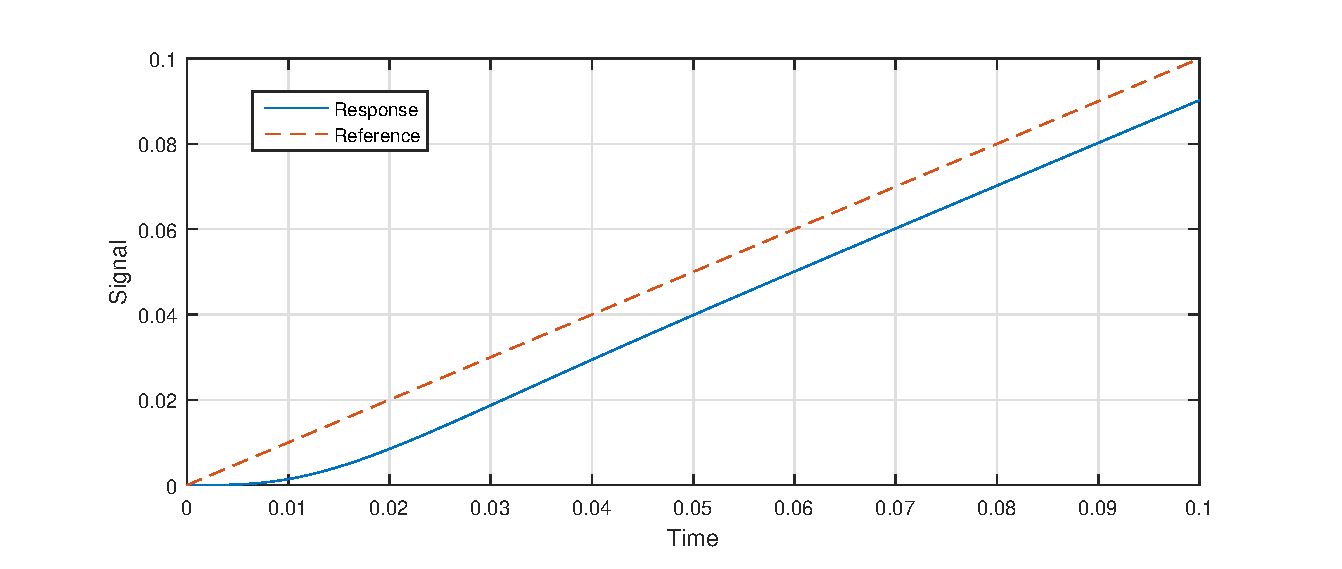
\includegraphics[width=\linewidth]{Plots/slope_delay1.eps}
  \end{center}
  \caption{System reaction under a slope signal.}
  \label{fig:slope}
\end{figure}

While overshoot and slope delay can only speak one aspect of the system, ISE is a rather comprehensive criterion. If reference signal is $r(t)$ and output of the closed loop system is $y(t)$, ISE is defined as $$ ISE = \int_{0}^{\tau} (r(t)-y(t))^2dt$$ where $\tau$ is the period of the signal if input is periodic. With such a layout, ISE constraint calls for transformation before it can be fitted into the context of GP. In \cite{malmquist2015tool} a method based on Fourier transform is used, in which a signal is at first decomposed as a series of harmonics and output of those harmonics can be calculated by checking the frequency response of the system. System reaction can be estimated by combining harmonic output together. Another approach use discretized state space model instead. Both methods can provide sufficient and precise information of the system reaction. In terms of efficiency, since the current software framework is running in Matlab and matrix is preferred in the software, state-space approach annihilate its counterpart. Therefore, the latter approach is illustrated here. In other context, harmonic approach might perform better instead.

The transfer function $G_{\text{cl}}(s)$ has all desired poles since it is  obtained by pole placement method. Suppose it is strictly proper and the transfer function is 
$$\frac{Y(s)}{R(s)}=G_{\text{cl}}(s)=\frac{b_1s^{n-1}+b_2s^{n-2}+ \cdots +b_n}{s^n+a_1s^{n-1}+ \cdots + a_n}=\frac{N_\text{cl}(s)}{D_{\text{cl}}(s)}$$ where $Y(s)$ and $R(s)$ are Laplace transform of output $y(t)$ and $r(t)$ respectively and $n \in \mathbf{N_{++}}$. Its state space model, by following the method from \cite{astrom2010feedback}, is given by 
\begin{equation}\label{eq:st_sp}
\begin{aligned} 
\dot{\mathbf{x}}&=A_{n \times n}\mathbf{x}+B_{n \times 1}r\\
y&=C_{1 \times n} \mathbf{x}
\end{aligned} 
\end{equation}
The state variable $\mathbf{x}$ is defined as $$\mathbf{x}=\left[\begin{array}{c}v^{(n)}\\ \vdots \\v^{(1)}\\v \end{array}\right]$$ where Laplace transform of $v$ fulfills $\sfrac{Y(s)}{V(s)}=N_{\text{cl}}(s)$ and $\sfrac{R(s)}{V(s)}=D_{\text{cl}}(s)$. The matrices of the model is given by $$ A_{n \times n} = 
 \left[\begin{array}{ccccc}
  -a_1 & -a_2 & \cdots & -a_{n-1} & -a_n \\
  1 &	0 & \cdots & 0 & 0 \\
  0 &	1 & \cdots & 0 & 0 \\
  \vdots  &   & \ddots & & \vdots  \\
  0 & 0 &  & 1 & 0
 \end{array}\right] $$ $$ B_{n \times 1} = \left[\begin{array}{c}1\\0\\ \vdots \\ 0 \end{array}\right]\; \text{and}\; C_{1 \times n}= \left[\begin{array}{c}b_1\\b_2\\ \vdots \\ b_n \end{array}\right]^T $$
 
By applying forward mode, the continuous state space model can be  discritized as \ref{eq:st_sp_d} where $t_s$ is sampling time. The whole trajectory can be expressed as a function of design variables and desired poles. Then ISE can be calculated based on trajectory. \begin{equation}\label{eq:st_sp_d}
\begin{aligned} 
\mathbf{x}(n)& =(t_sA_{n \times n}+I_n)\mathbf{x}(n-1)+t_sB_{n \times 1}r(n-1)\\
y(n) & = C_{1 \times n} \mathbf{x}(n)
\end{aligned} 
\end{equation} 

Those three criteria can become posybonials by following above approach. They can be applied independently or combined together to guarantee good dynamics of the designed system. There are plenty of evaluation criteria for system dynamics which can be introduced to this design approach, most of which have very complex format. Therefore, in order to apply them for optimization, those criteria need to be modified or even simplified to be posynomials.
%%%%%%%%%%%%%% end Optimization approach %%%%%%%%%%%

%%%%%%%%%%%%%% begin Optimization approach %%%%%%%%%
\section{Case Study}

\begin{figure}[]
  \begin{center}
    %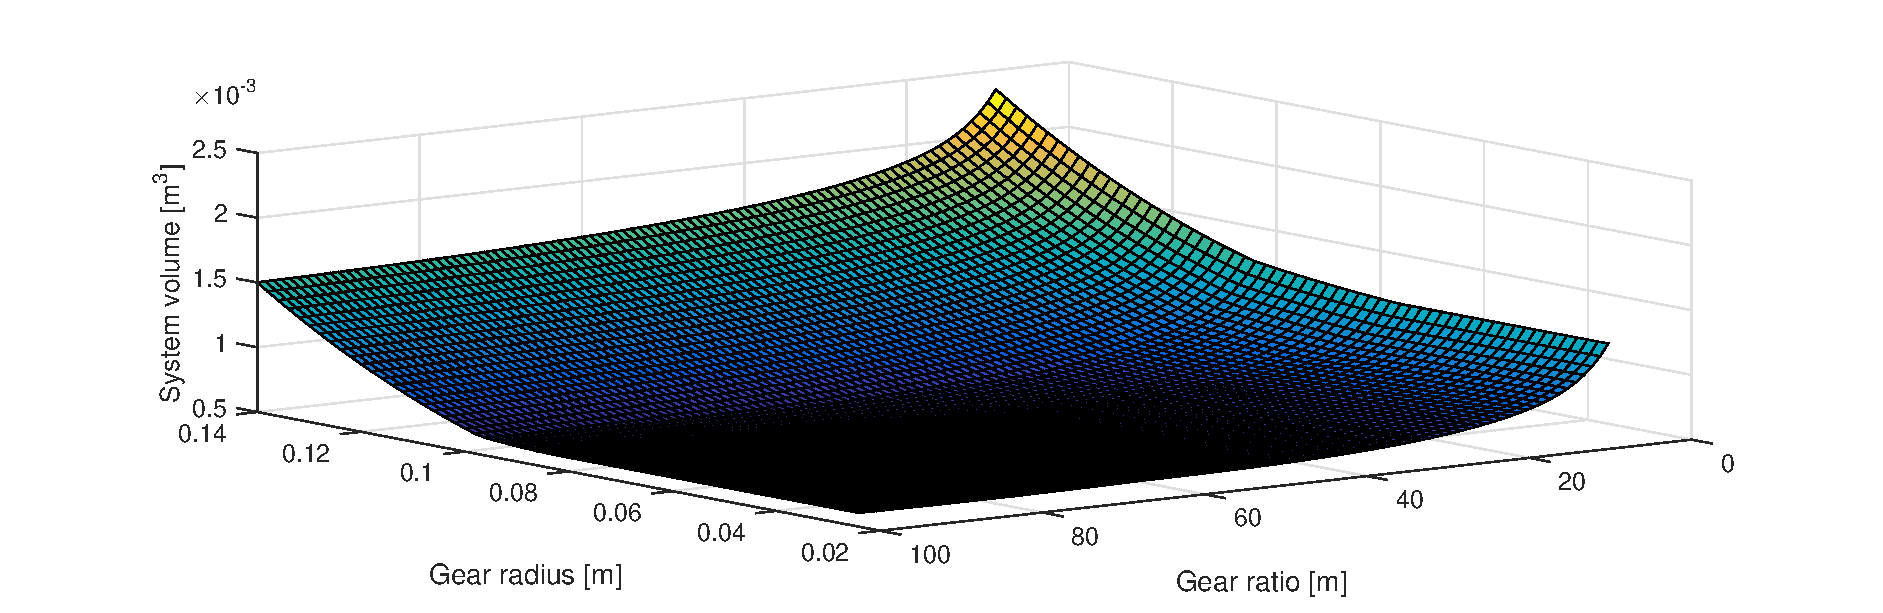
\includegraphics[width=\linewidth]{Plots/3Dplot_convex_static_mediumQ.eps}
    \missingfigure[figwidth=\linewidth]{Testing a long text string}
  \end{center}
  \caption{Mechatronics servo system consisting of a motor and planetary gear which serves as the design case.}
  \label{fig:CaseSystem}
\end{figure}

The physical system studied in our case is a mechatronic servo system consisting of a motor, a shaft and two planetary gear stages; as shown in figure \ref{fig:CaseSystem}. Both the static and dynamic models for different components have been previously developed by Roos and Malmquist. The load inertia, $J_{\text{load}}$, for the presented design case is as 1.1$kg/m^2$ and the chosen load profile can be viewed in Figure \ref{???}. This scenario is equivalent to the one presented by Malmquist in order to perform a fair comparison. The dimensioning factor introduced in the dynamic model is according to Malmquist$'$s method applied to all the valid results from the static model, while in our case, the dimensioning factor is only calculated for the optimum from the static models.

%From figure ??? [[[[we can see]]] that the peak torque is $T_{peak}=191.4 N/m$ and the root mean square (RMS) value of torque $T_{RMS} = 49.39 N/m$. Similarly, the optimization objective is still the system volume.    

\subsection*{Models}
This section will focus on how to convert the excising mathematical models of the components in our design case to geometrical forms which can be analysed in the CVX software. 
\subsubsection*{Motor}
The motor model was derived by Roos\cite{roos2007} based on the constraint that the rated torque should be no less than the expected RMS torque according to
\begin{equation} \label{eq:cs1}
T_{\text{m,rated}} \geq \tilde{T}_{\text{m}}.
\end{equation}
Furthermore, Roos derived the rated torque of the motor considering mechanical, magnetic and thermal effects as
\begin{equation} \label{eq:cs2}
T_{\text{m,rated}}=C_{\text{m}}l_{\text{m}} r_{\text{m}}^{2.5}
\end{equation}
where $C_{\text{m}}$ is a constant for a specific motor type and cooling condition, $l_{\text{m}}$ is the motor length and $r_{\text{m}}$ the radius of the stator. The RMS torque required from the motor is derived by propagating the load torque $T_{\text{l}}$ through the planetary gear with gear ratio $n$
\begin{equation} \label{eq:cs3}
\tilde{T}_{\text{m}}=\sqrt{\frac{1}{\tau}\int_0^\tau ((C_{\text{mj}}l_{\text{m}} r_{\text{m}}^{4}+J_{\text{m}})\ddot{\varphi}_{\text{m}}+\frac{T_{\text{l}}}{n})^2  \mathrm{d} t}
\end{equation}
where $C_{\text{mj}}$ is constant for a specific motor type and derived from a reference motor of the same type, $J_{\text{m}}$ is the rotor inertia ${\varphi}_{\text{m}}$ is the angular position of the output shaft.
Rewriting the equation \ref{eq:cs1} by combining equation \ref{eq:cs2} and \ref{eq:cs3} results in
\begin{equation} \label{eq:cs4}
C_{\text{m}}l_{\text{m}} r_{\text{m}}^{2.5}\geq \sqrt{\frac{1}{\tau}\int_0^\tau ((C_{\text{mj}}l_{\text{m}} r_{\text{m}}^{4}+J_{\text{m}})\ddot{\varphi}_{\text{m}}+\frac{T_{\text{l}}}{n})^2  \mathrm{d} t}.
\end{equation}
Hence, the geometric form of this constraint can then be stated as
\begin{equation} \label{eq:cs5}
\frac{n_{\text{j}}^2 n^2 C_{\text{mj}}^2 T_{\text{rms}}^2 r_{\text{m}}^3}{J_{\text{load}}^2} + \frac{2 n_{\text{j}} C_{\text{mj}} T_{\text{rms}}^2}{J_{\text{load}} r_{\text{m}} l_{\text{m}}} + \frac{T_{\text{rms}}^2}{n^2 l_{\text{m}}^2 r_{\text{m}}^5}\leq C_{\text{m}}^2
\end{equation}
where $n_{\text{j}}$ is defined as $\frac{C_{\text{mj}}l_{\text{m}} r_{\text{m}}^{4}+J_{\text{m}}}{C_{\text{mj}}l_{\text{m}} r_{\text{m}}^{4}}$ and approximated as 10/9. 

A complementary constraint for the motor model is form factor constraint
\begin{equation} \label{eq:cs6}
0.5 \leq \frac{l_{\text{m}}}{r_{\text{m}}} \leq 5
\end{equation}

The dynamic model of the motor is derived as
\begin{equation} \label{eq:cs7}
K_{\text{t}}i= \frac{T_{\text{l}}}{n} + J_{\text{m}}\ddot{{\varphi}}_{\text{m}}
\end{equation}
where $K_{\text{t}}$ is the constant and $i$ is the electric current.


\subsubsection*{Planetary gear}
A planetary gear consisting of a sun gear, three planet gears and a ring gear is used in the servo system //Nescessary?//instead of a spur gear since the volume of the planetary gear is less than a spur gear when transmitting the same torque////. The main constraints on the planetary gear are bending stress in the root of a gear teeth and Hertzian pressure at the teeth contact surfaces. However, if the number of the sun gear teeth is small and/or the the gears are made from ductile steel, the dominant constraint would be the Herzian pressure. Every teeth surface needs to fulfil 
\begin{equation} \label{eq:cs8}
r_{\text{g}}^2b \geq Z_{\text{H}}^2 Z_{\text{M}}^2 Z_{\epsilon} K_{\text{H} \alpha} K_{\text{H} \beta} \frac{T_{\text{l}}(n-1)^2}{6(n-2)\sigma_{\text{H,max}}^2}.
\end{equation}
according to Roos. Applying the standard parameters defined in Roos$'$ work, equation \ref{eq:cs8} can be simplified as
\begin{equation} \label{eq:cs9}
r_{\text{g}}^2b \geq 4\cdot10^{10} \cdot C_{\text{gr}}^2\frac{T_{\text{l}}(n-1)^2}{(n-2)\sigma_{\text{H,max}}^2}
\end{equation}
where $C_{\text{gr}}$ is the ratio of the outer gear radius and the gear$'$s pitch radius; $\sigma_{\text{H,max}}$ is the maximum allowed flank pressure given by
\begin{equation} \label{eq:cs10}
\sigma_{\text{H,max}}=\frac{\sigma_{\text{H,lim}}}{SF}
\end{equation}
where $\sigma_{\text{H,lim}}$ is the maximum allowed Herzian pressure for the particular gear material and $SF$ is the safe factor.

The geometric form to replace the equation \ref{eq:cs9} is expressed as
\begin{equation} \label{eq:cs11}
\frac{(n-1)^2}{(n-2)} \approx n+\sum_{i=0}^{\infty} \frac{1}{n}\times(\frac{2}{n})^i = \frac{(n-1)^2-(\frac{2}{n})^i}{n-2}
\end{equation}

The equation \ref{eq:cs11} holds when the term $(\frac{2}{n})^i$ is sufficiently small, which can be satisfied by $n \gg 2$ and the number of the sum terms $i$ is sufficiently large. 

\subsubsection*{Shaft}
The static model for the shaft is derived from the classic solid mechanics. The following equations are from Collins[????]
\begin{equation} \label{eq:cs12}
r_{\text{s}} = \sqrt[3]{\frac{2\tilde{T}_{\text{s,out}}}{\tau_{\text{s,max}} \pi}}
\end{equation}
\begin{equation} \label{eq:cs13}
J_{\text{s}} = \frac{\pi r_{\text{s}}^4}{2}
\end{equation}
\begin{equation} \label{eq:cs14}
G = \frac{E}{2(1+\nu)}
\end{equation}
\begin{equation} \label{eq:cs15}
k = \frac{GJ_{\text{s}}}{l}
\end{equation}
where $r_{\text{s}}$ is the shaft radium, $\tilde{T}_{\text{s,out}}$ is the maximum transferred torque, $\tau_{\text{s,max}}$ is the maximum permissible shear stress, $J_{\text{s}}$ is the shaft polar moment of inertia, $G$ is the shear modulus, $E$ is Young$'$s modulus, $\nu$ is Poisson$'$s ratio, $l$ is the length and $k$ is the stiffness of the shaft.
 
The shaft dynamic behavior is approximated as a spring-damper model. The equations are derived as
\begin{equation} \label{eq:cs16}
\frac{1}{2}J_{\text{s}}\ddot{\varphi}_{\text{s,in}} = T_{\text{s,in}}-k(\varphi_{\text{s,in}}-\varphi_{\text{s,out}})-d(\dot{\varphi}_{\text{s,in}}-\dot{\varphi}_{\text{s,out}})
\end{equation}
\begin{equation} \label{eq:cs17}
\frac{1}{2}J_{\text{s}}\ddot{\varphi}_{\text{s,out}} = k(\varphi_{\text{s,in}}-\varphi_{\text{s,out}})+d(\dot{\varphi}_{\text{s,in}}-\dot{\varphi}_{\text{s,out}})-T_{\text{s,out}}.
\end{equation}
\subsubsection*{Load}
Load does not have a static model as a physical component does. However, the dynamic model exists and derived as
\begin{equation} \label{eq:cs18}
J_{\text{l}}\ddot{\varphi}_{\text{l}} = T_{\text{l}}
\end{equation}
where $J_{\text{l}}$ is the load inertia and $T_{\text{l}}$ is the load torque.  
\subsection*{Results Comparision}
After arranging the static constraints of different components to geometric form, the physical system would be optimized for volume from the aspects of both static and dynamic using CVX toolbox. The optimization results as well as computing time would be recorded to be compared with Malmquist$'$ work. 
After running CVX, the values for different design variables as well as computing time are obtained and recorded along with those from GA  in table????? and table ?????
table?                                     
\begin{table}[h]
\caption{Static model results}
\label{sta}
\begin{center}
\begin{tabular}{|c||c||c|}
\hline
Comparison Item & Convex Optimization & Genetic Algorithm\\
\hline
$Three$ & $Four$ & $Four$\\
\hline
$Three$ & $Four$ & $Four$\\
\hline
$Three$ & $Four$ & $Four$\\
\hline
$Three$ & $Four$ & $Four$\\
\hline
$Three$ & $Four$ & $Four$\\
\hline
\end{tabular}
\end{center}
\end{table}

In dynamic model, ISE is calculated by applying the discrete state space method mentioned above to the closed loop transfer function with all the poles chosen at $-150$ beforehand. The expression for ISE is $k$, which only depends on $k$ since $k$ is the only design variable contained in the numerator of the closed loop transfer function. As observed, the expression yields a parabolic curve regarding $\frac{1}{k}$. An explanation could be that ISE increases as $k$ decreases since a softer shaft causes bigger overshoot when $k<k_o$ and ISE increases as $k$ increases since a stiffer shaft causes bigger lag time when $k>k_o$.
It can be seen that convex optimization returns the results with allowed error while the computing time is much shortened compared with genetic algorithm. 
\begin{table}[h]
\caption{Dynamic model results}
\label{dyn}
\begin{center}
\begin{tabular}{|c||c||c|}
\hline
Comparison Item & Convex Optimization & Genetic Algorithm\\
\hline
$Three$ & $Four$ & $Four$\\
\hline
$Three$ & $Four$ & $Four$\\
\hline
$Three$ & $Four$ & $Four$\\
\hline
$Three$ & $Four$ & $Four$\\
\hline
$Three$ & $Four$ & $Four$\\
\hline
\end{tabular}
\end{center}
\end{table}

\begin{figure}[t]
  \begin{center}
    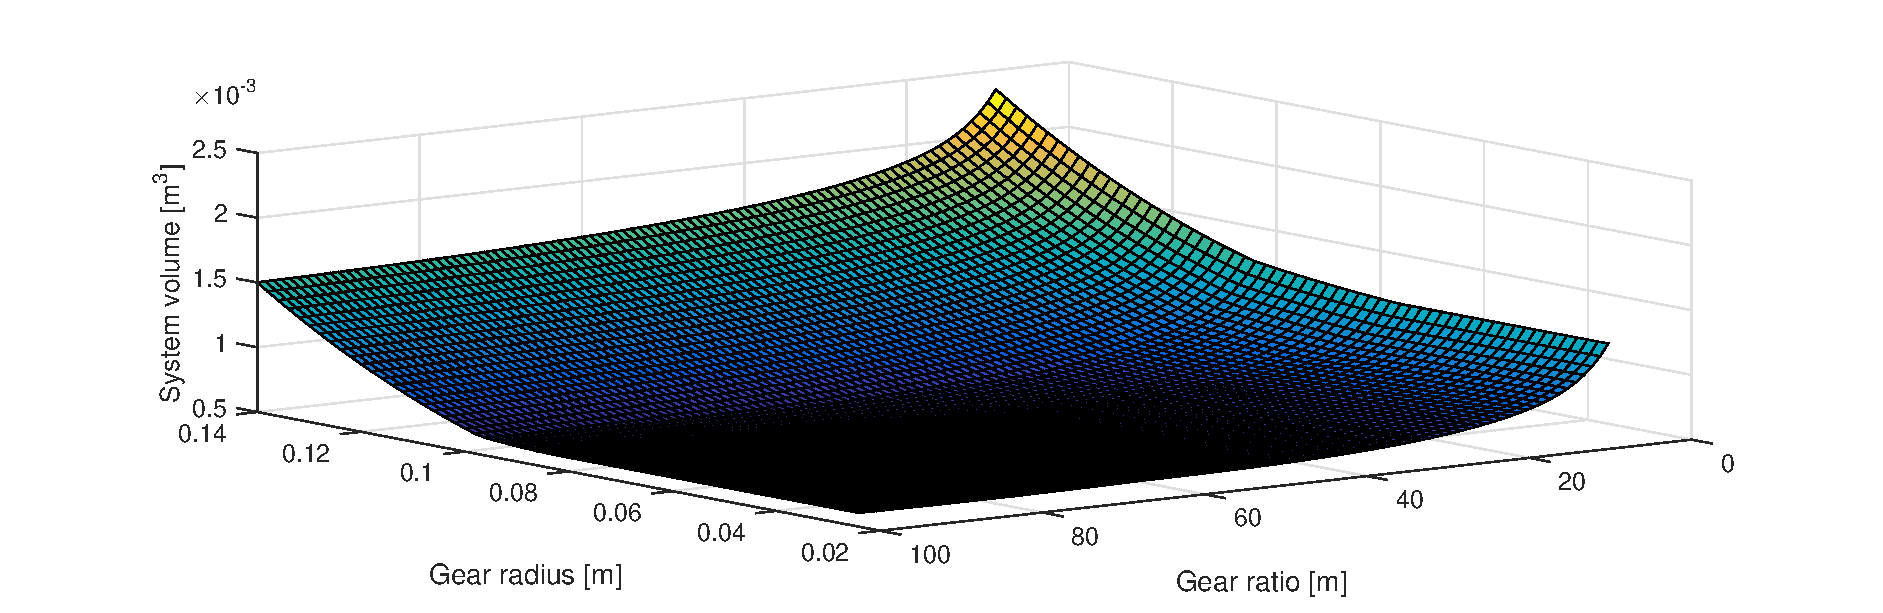
\includegraphics[width=\linewidth]{Plots/3Dplot_convex_static_mediumQ.eps}
  \end{center}
  \caption{Optimal volume for static case with varying gear radius and gear ratio.}
  \label{fig:static3D}
\end{figure}



%%%%%%%%%%%%%% end Optimization approach %%%%%%%%%%%

%%%%%%%%%%%%%% begin conclusion %%%%%%%%%%%
\section{Conclusion}
Conclusion...
%%%%%%%%%%%%%% end conclusion %%%%%%%%%%%%%

%%%%%%%%%%%%%% begin acknowlegement %%%%%%%
\section*{Acknowledgment}
%%%%%%%%%%%%%% end acknowlegement %%%%%%%%%

%%%%%%%%%%%%%% begin acknowlegement %%%%%%%


%\bibitem{IEEEhowto:kopka}
%H.~Kopka and P.~W. Daly, \emph{A Guide to \LaTeX}, 3rd~ed.\hskip 1em plus
 % 0.5em minus 0.4em\relax Harlow, England: Addison-Wesley, 1999.

%\end{thebibliography}
%%%%%%%%%%%%%% end acknowlegement %%%%%%%%%

%\nocite{*}
\bibliographystyle{ieeetran}
\bibliography{./Contents/References/references}

\end{document}



%\section*{Handy Examples}

%\subsection*{Figure example}

%\begin{figure}[!t]
%\centering
%\includegraphics[width=0.25\textwidth]{./Contents/myFigure.png}
%\caption{Simulation results for the network.}
%\label{fig_sim}
%\end{figure}

%\subsection{Table example}
%\begin{table}[!t]
%% increase table row spacing, adjust to taste
%\renewcommand{\arraystretch}{1.3}
% if using array.sty, it might be a good idea to tweak the value of
% \extrarowheight as needed to properly center the text within the cells
%\caption{An Example of a Table}
%\label{table_example}
%\centering
%% Some packages, such as MDW tools, offer better commands for making tables
%% than the plain LaTeX2e tabular which is used here.
%\begin{tabular}{|c||c|}
%\hline
%One & Two\\
%\hline
%Three & Four\\
%\hline
%\end{tabular}
%\end{table}




